\documentclass{ctexart}
\usepackage{PhysicalChemistryNote}

\begin{document}\pagestyle{plain}
\noindent\tbf{\LARGE 7C 反应机理与速率方程的推导}\vspace{15pt}\\
\indent 化学反应在大多数情况下并不是一蹴而就的.例如葡萄糖\ce{C6H12O6}在你的身体里被氧化的过程:%
\ce{C6H12O6 + 6O2 -> 6CO2 + 6H2O}.显然,让一个\ce{C6H12O6}分子与六个\ce{O2}分子一步到位地生成%
六个\ce{CO2}分子与六个\ce{6H2O}分子是不大现实的,这需要所有\ce{O2}同时以合适的角度接近并发生反应,%
这一概率是非常低的.事实上我们知道,这一反应,乃至绝大多数反应都是通过数个步骤进行的,%
这些步骤构成了我们所讲的反应机理,并且也密切影响着反应的速率.\vspace{12pt}\\
\Section{7C.1 基元反应}
\Part{基元反应}
\indent 在前言中,我们说大部分反应都是通过数个步骤进行的.这些简单而基本的步骤就是我们所说的\tbf{基元反应}.
\begin{definition}[7C.1.1 基元反应]
    \tbf{基元反应}(或称\tbf{基本反应}),顾名思义,即最简单的化学反应步骤,是一个或多个化学物种直接作用,一步(即通过单一过渡态)转化为反应产物的过程.
\end{definition}
下面是几个常见的基元反应:
\begin{tightcenter}
    \ce{H. + Br2 -> HBr + Br.}\\
    \ce{CH3I + Cl- -> CH3Cl + I-}\\
    \ce{I2 -> 2I.}
\end{tightcenter}
可以看到,参与基元反应的物质并不一定是稳定的化合物,也可能是自由基等不稳定物种.并且,参与反应的分子数各不相同.
\begin{theorem}[7C.1.2 基元反应的分子数]
    基元反应的\tbf{分子数}是指参与基元反应的分子数.\\
    在\tbf{单分子反应}中,单个分子振动分解或发生重排.\\
    在\tbf{双分子反应}中,参与反应的两个分子以合适的方式碰撞,发生能量交换,键的生成和断裂等过程.\\
    一般而言,三分子反应已经很少见,而分子数大于等于四的基元反应几乎不存在.
\end{theorem}
基元反应,正由于其简单的特征,速率方程也十分简洁.
\begin{theorem}[7C.1.3 基元反应的速率方程]
    单分子基元反应对反应物为一级,其速率(以\ce{A -> P}为例)为$v=k\con{A}$.\\
    双分子基元反应对每个反应物都为一级(如果反应物相同就为二级),其速率(以\ce{A + B -> P}为例)为$v=k\con{A}\con{B}$,%
    或(以\ce{2A -> P}为例)为$v=k\con{A}^2$.
\end{theorem}
我们可以对上面的结论做定性的解释.%
在一定温度下,具有适合的能量的分子在总体中占的比例是一定的.因此,参与基元反应的物质的浓度越高,%
具有适合的能量的分子的浓度就越高,反应速率也就越快,并且对每个参与反应的分子的浓度都应当%
成正比例关系.\vspace{4pt}\\
\Part{微观可逆性原理和精细平衡原理}
\indent 直觉地来看,如果将描述物质运动的方程中的时间$t$和速度$v$替换成其负值,并不影响运动方程%
的成立.因此,运动的过程是可以通过恰好相反的方向进行的,而它们遵守相同的物理规律.这就是力学中的\tbf{时间反演对称性}%
\footnote{说得粗糙一些,这和时间倒流在某种程度上是一致的.如果你看过Christopher Nolan执导的电影《信条》,可能对这样的现象会有更为直观的认识.}.
\begin{hint}
    这一“直觉”事实上在经典力学和量子力学中都可以被证明,但由于涉及到一些复杂的物理知识,故在此并不给出.\\
    需要注意的是,由于我们在这里讨论的仅仅是单个或少数几个物体(即分子),因此尚不具有统计意义.%
    这要与热力学第二定律做区分.\\
    你可以简单地认为,力学肯定的是微观过程的可逆性,而统计物理学(以及热力学)肯定的是宏观过程的不可逆性,%
    两者讨论的范畴并不相同,因此也没有矛盾之处.
\end{hint}
以上我们从力学的角度讨论了时间反演对称性.它告诉我们,化学过程中反应的微粒服从力学方程(如基元反应中反应物微粒单次碰撞行为),%
则在正,逆反应过程中所经历的途径是相同的,逆过程要经历正过程的所有状态,就像一部电影从后往前倒过来放映,%
片中的一切动作是正常放映时动作的完全逆转;同时,在沿着反应坐标移动形成并最后解体的活化络合物的组成和结构在两个方向上是相同的,只不过动量的符号相反.%
由此,我们可以提出时间反演对称在化学动力学中的表述.
\begin{theorem}[7C.1.4 微观可逆性原理]
    如果一个正反应是基元反应,那么它的逆反应也是基元反应,且正逆反应具有相同的活化络合物(即中间体).
\end{theorem}
微观可逆性原理对假设反应厉程有明显的制约:它要求设想的反应机理中任一基元反应的逆反应不应是不可能的反应.%
如四乙基铅的气相分解反应:\ce{Pb(C2H5)4 -> Pb + 4C2H5.},逆反应是不可能发生的五分子反应,所以该反应不可能是基元反应.\\
\indent 到目前为止,我们似乎仍未考虑反应达到平衡的情形.此时,总体正反应和逆反应的速率相等,%
各物质的浓度不再随时间变化.那么具体到每个基元反应上又是何种情况呢?%
为此,人们提出了精细平衡原理.
\begin{theorem}[7C.1.5 精细平衡原理]
    平衡时,宏观体系中每一个基元反应的速率一定等于其逆反应的速率.%
    这一定理也可以表述为:平衡时,每个对峙反应的速率都相同.
\end{theorem}
在化学动力学的范畴中,这也是一条可以被证明的定理.因此,这从根本上否定了平衡时存在单向不可逆循环的存在.%
每个基元反应必然存在其逆反应,且平衡时正逆反应的速率相等.%
我们将在之后看到精细平衡原理对反应机理的限制.\\
\indent 最后,需要说明的是尽管基元反应都存在逆反应,但很多基元反应的逆反应的速率非常缓慢,以至于可以忽略不计,%
因此我们近似地认为这些反应是不可逆的.这与我们在\tbf{5B.3.5}中说到的一致,即在动力学中,可逆是绝对的,不可逆是相对的.\vspace{12pt}\\
\Section{7C.2 连续反应动力学}
\Part{两步连续反应的积分速率方程}
\indent 基元反应最简单的组合方式就是连续地发生,通过几个连续的步骤完成反应.例如\ce{^{239}U}衰变为%
\ce{^{239}Pu},就是通过下面的连续$\beta$衰变进行的:
\begin{tightcenter}
    \ce{^{239}U ->T[$t_{1/2}=23.5$ min] ^{239}Np ->T[$t_{1/2}=2.35$ d] ^{239}Pu}
\end{tightcenter}
现在,我们尝试用数学方法推导最简单的连续反应——两步连续反应的积分速率方程.
\begin{derivation}
    考虑连续反应
    \begin{tightcenter}
        \ce{A ->T[$k_1$] I ->T[$k_2$] P}
    \end{tightcenter}
    对于\ce{A}而言,它的消耗是一个一级反应,满足
    \[\con{A}=\con{A}_0\e^{-k_1t}\]
    而\ce{I}满足
    \[\dfrac{\di\con{I}}{\di t}=k_1\con{A}-k_2\con{I}\]
    代入$\con{A}$的表达式即有
    \[\dfrac{\di\con{I}}{\di t}+k_2\con{I}=k_1\con{A}_0\e^{-k_1t}\]
    这是一个一阶线性常微分方程.我们已经讲过它的解法,即常数变易法.该方程对应的齐次方程
    \[\dfrac{\di\con{I}}{\di t}+k_2\con{I}=0\]
    的通解为
    \[\con{I}=C\e^{-k_2t}\]
    令$\con{I}=C(t)\e^{-k_2t}$,代入原方程即有
    \[C'(t)\e^{-k_2t}=k_1\con{A}_0\e^{-k_1t}\]
    于是
    \[C'(t)=k_1\con{A}_0\e^{\left(k_2-k_1\right)t}\]
    如果$k_1\neq k_2$,那么积分可得
    \[C(t)=\dfrac{k_1\con{A}_0}{k_2-k_1}\e^{\left(k_2-k_1\right)t}+I\]
    其中$I$为待定的积分常数.代回$\con{I}$的表达式就有
    \[\con{I}=\dfrac{k_1\con{A}_0}{k_2-k_1}\e^{-k_1t}+I\e^{-k_2t}\]
    由于起始是并没有中间产物\ce{I}的产生,因此$t=0$时$\con{I}=0$.代入上式即可得积分常数,整理可得
    \[\con{I}=\dfrac{k_1\con{A}_0}{k_2-k_1}\left(\e^{-k_1t}-\e^{-k_2t}\right)\]
    从而反应的速率(这里以生成\ce{P}的速率计)为
    \[v=\dfrac{\di\con{P}}{\di t}=k_2\con{I}=\dfrac{k_1k_2\con{A}_0}{k_2-k_1}\left(\e^{-k_1t}-\e^{-k_2t}\right)\]
    由于$\con{A}+\con{I}+\con{P}=\con{A_0}$总是成立,于是
    \[\con{P}=\left(1+\dfrac{k_1\e^{-k_2t}-k_2\e^{-k_1t}}{k_2-k_1}\right)\con{A}_0\]
    这就是两步连续反应的速率方程.
\end{derivation}
\begin{theorem}[7C.2.1 两步连续反应的积分速率方程]
    连续反应\ce{A ->T[$k_1$] I ->T[$k_2$] P}的积分速率方程为
    \[\con{P}=\left(1+\dfrac{k_1\e^{-k_2t}-k_2\e^{-k_1t}}{k_2-k_1}\right)\con{A}_0\]

\end{theorem}
至于更多步的连续反应,虽然在理论上不过是多次应用常数变易法解微分方程,但其计算的复杂程度却是迅速增长的\footnote{但这似乎并不妨碍某些丧心病狂的出题人考察多步连续反应的积分速率方程.}.%
因此大多数情况下,我们也不要求连续反应的精确的积分速率方程,而是采取合理的近似以简化计算.\vspace{4pt}\\
\Part{稳态近似}
\indent 当反应机理变得更加复杂(例如存在逆反应或多步连续反应时),微分方程可能就没有显式的解,%
精确求解这样的体系也会使得计算难度大幅增加.因此我们需要想办法做一些合理的近似以简化计算.%
为此,我们先观察以下情况下两步连续反应的各物质浓度随时间变化的图像.
\begin{figure}[H]
    \centering\documentclass{standalone}
\usepackage{PhysicalChemistryNote}
\begin{document}
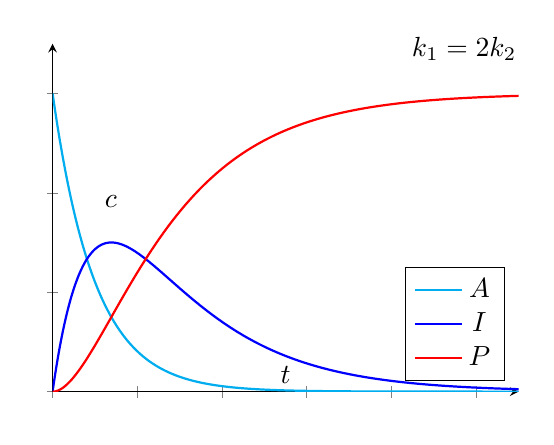
\begin{tikzpicture}
    \begin{axis}[
        title = {$k_1=2k_2$},
        title style={at={(0.75,1)},anchor=north west},
        width = 7.5cm,
        height = 6cm,
        legend pos = south east,
        x label style={at={(axis description cs:0.5,0.1)},anchor=north},
        y label style={at={(axis description cs:0.125,0.5)},rotate=270,anchor=south},
        xlabel = {$t$},
        ylabel = {$c$},
        axis lines = left,
        ymax = 3.5,
        domain = 0:5.5,
        samples = 400,
        xticklabels={},
        yticklabels={}
    ]
    \addplot [thick, cyan] {3*e^(-2*x)};
    \addplot [thick, blue] {3*2*(e^(-x)-e^(-2*x))};
    \addplot [thick, red] {3*(1-(2*e^(-x)-e^(-2*x)))};
    \legend {$\con{A}$,$\con{I}$,$\con{P}$}
    \end{axis}
\end{tikzpicture}
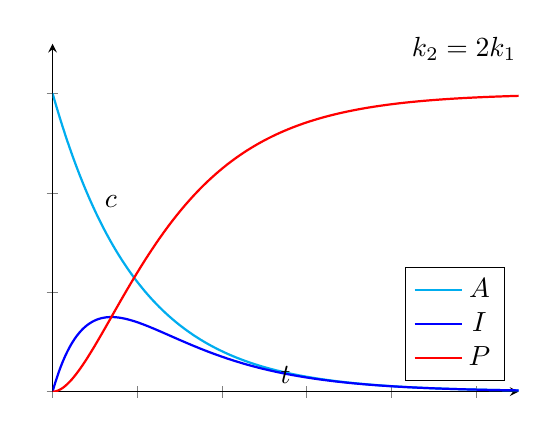
\begin{tikzpicture}
    \begin{axis}[
        title = {$k_2=2k_1$},
        title style={at={(0.75,1)},anchor=north west},
        width = 7.5cm,
        height = 6cm,
        legend pos = south east,
        x label style={at={(axis description cs:0.5,0.1)},anchor=north},
        y label style={at={(axis description cs:0.125,0.5)},rotate=270,anchor=south},
        xlabel = {$t$},
        ylabel = {$c$},
        axis lines = left,
        ymax = 3.5,
        domain = 0:5.5,
        samples = 400,
        xticklabels={},
        yticklabels={}
    ]
    \addplot [thick, cyan] {3*e^(-x)};
    \addplot [thick, blue] {3*(e^(-x)-e^(-2*x))};
    \addplot [thick, red] {3*(1-(2*e^(-x)-e^(-2*x)))};
    \legend {$\con{A}$,$\con{I}$,$\con{P}$}
    \end{axis}
\end{tikzpicture}
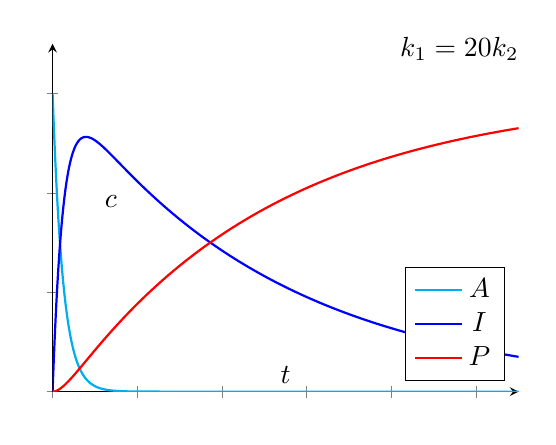
\begin{tikzpicture}
    \begin{axis}[
        title = {$k_1=20k_2$},
        title style={at={(0.725,1)},anchor=north west},
        width = 7.5cm,
        height = 6cm,
        legend pos = south east,
        x label style={at={(axis description cs:0.5,0.1)},anchor=north},
        y label style={at={(axis description cs:0.125,0.5)},rotate=270,anchor=south},
        xlabel = {$t$},
        ylabel = {$c$},
        axis lines = left,
        ymax = 3.5,
        domain = 0:5.5,
        samples = 400,
        xticklabels={},
        yticklabels={}
    ]
    \addplot [thick, cyan] {3*e^(-8*x)};
    \addplot [thick, blue] {3/7.6*8*(e^(-0.4*x)-e^(-8*x))};
    \addplot [thick, red] {3*(1+(0.4*e^(-8*x)-8*e^(-0.4*x))/7.6)};
    \legend {$\con{A}$,$\con{I}$,$\con{P}$}
    \end{axis}
\end{tikzpicture}
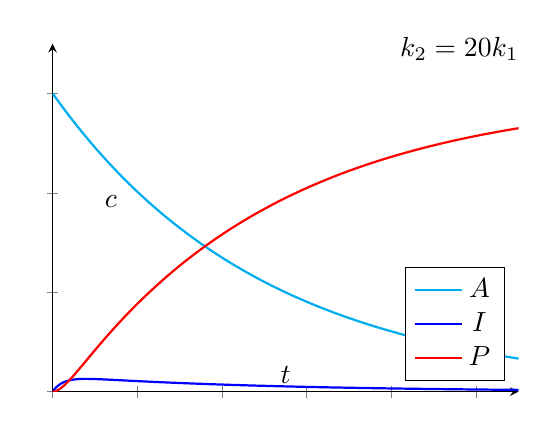
\begin{tikzpicture}
    \begin{axis}[
        title = {$k_2=20k_1$},
        title style={at={(0.725,1)},anchor=north west},
        width = 7.5cm,
        height = 6cm,
        legend pos = south east,
        x label style={at={(axis description cs:0.5,0.1)},anchor=north},
        y label style={at={(axis description cs:0.125,0.5)},rotate=270,anchor=south},
        xlabel = {$t$},
        ylabel = {$c$},
        axis lines = left,
        ymax = 3.5,
        domain = 0:5.5,
        samples = 400,
        xticklabels={},
        yticklabels={}
    ]
    \addplot [thick, cyan] {3*e^(-0.4*x)};
    \addplot [thick, blue] {3/7.6*0.4*(e^(-0.4*x)-e^(-8*x))};
    \addplot [thick, red] {3*(1+(0.4*e^(-8*x)-8*e^(-0.4*x))/7.6)};
    \legend {$\con{A}$,$\con{I}$,$\con{P}$}
    \end{axis}
\end{tikzpicture}
\end{document}
\end{figure}
当$k_1>k_2$时,可以发现反应\ce{A}迅速消耗,同时生成了一定量的中间体\ce{I},再转化为产物\ce{P}.%
而当$k_2\gg k_1$时,可以看到在相当长的一段时间里,$\con{I}$的浓度变化不大(并且相当的低),%
我们可以从前面的结果对这一猜测进行证明.
\begin{derivation}
    首先,直观地来说,如果$k_2\gg k_1$,这说明第二步反应的速率相对于第一步反应更快.因此,在反应进行不久后,%
    我们可以认为一定时间内\ce{A}转化为\ce{I}后立即转化为\ce{P}.在这段时间内,$\con{I}$随时间变化不大,%
    即$\dfrac{\di\con{I}}{\di t}\sim0$,于是
    \[k_2\con{I}=k_1\con{A}\]
    于是
    \[\con{I}=\dfrac{k_1}{k_2}\con{A}\]
    这表明$\con{I}$与$\con{A}$成正比例关系,比例系数为$\dfrac{k_1}{k_2}$.\\
    现在从定量的角度说明这一结果.我们有
    \[\dfrac{\con{I}}{\con{A}}=\dfrac{k_1}{k_2-k_1}\left(1-\e^{\left(k_1-k_2\right)t}\right)\]
    如果$k_2\gg k_1$,那么$k_1-k_2\ll0$.于是$1-\e^{\left(k_1-k_2\right)t}\sim1$.又
    \[\dfrac{k_1}{k_2-k_1}\sim\dfrac{k_1}{k_2}\]
    从而
    \[\dfrac{\con{I}}{\con{A}}=\dfrac{k_1}{k_2}\]
    尽管在作此近似后,$\con{I}$随$\con{A}$变化而变化,但由于比例系数$\dfrac{k_1}{k_2}$很小,因此我们的假设$\dfrac{\di\con{I}}{\di t}\sim0$仍然是成立的.%
    由此,我们可以得到
    \[\dfrac{\di\con{P}}{\di t}=k_2\con{I}=k_1\con{A}\]
    这一式子与\ce{A}直接生成\ce{P}的积分速率方程相同.%
    在\tbf{7C.2.1}令$k_2\gg k_1$,亦可以得到相同的结果.
\end{derivation}
这就是在动力学中非常重要的\tbf{稳态近似}.
\begin{theorem}[7C.2.2 稳态近似]
    连续反应中的不稳定中间体的净生成速率可以近似视作$0$.%
    在经历反应的\tbf{诱导期}(即中间体\ce{I}在反应初始时的生成)后,在反应的主要阶段,其浓度变化都很小.
\end{theorem}
需要说明的是,这里的“浓度变化很小”并不指的是$\con{I}$不变,而是$\dfrac{\di\con{I}}{\di t}$视作$0$.%
尽管这两个说法看起来有点矛盾,不过我们始终应当将目光放在产物和反应物等主要物质上,因此主要是通过稳态近似得出联系几种物质的等量关系,%
而非关注中间体本身的浓度.\\
\indent 前面推导中的\ce{I}就是不稳定中间体,它被消耗的速率常数$k_2$远大于生成的速率常数$k_1$,%
因而相对的难以生成而容易消耗.我们将在\tbf{7E}中讲述速率常数与活化能的关系,%
进而说明满足这样条件的中间体\ce{I}的能量相对而言比较高.\\
\indent 我们所说的不稳定中间体,一般而言可以根据你的化学知识储备判断,比如各种自由基和不稳定的分子等等.\\
\indent 应用稳态近似,我们可以将体系中所有不稳定中间体所对应的微分方程变为一个确定的等量关系,从而大大简化计算.%
我们将在本节之后的例子和本章的习题中反复应用这一重要定律.\vspace{4pt}\\
\Part{速率控制步骤}
\indent 尽管本小节放在\tbf{7E}介绍似乎更为合适,但我们仍然可以从连续反应的积分速率方程中得出一些有用的结论.%
前面我们已经知道,当$k_2\gg k_1$时,利用稳态近似可得
\[\dfrac{\di\con{P}}{\di t}=-\dfrac{\di\con{A}}{\di t}\]
即\ce{A}消耗的速率与\ce{P}生成的速率相等.这表明反应的速率大体上由第一步的速率决定.
\begin{hint}
    认识到在稳态近似后\ce{A -> I}和\ce{I -> P}的速率相同是十分重要的:与\ce{A}相比,%
    \ce{I}的浓度是如此之低,以至于尽管$k_2\gg k_1$,这两步反应的速率仍然几乎相同.\\
    因此,通常所说的“第一步慢,第二步快,所以第一步是决速步”是有问题的.实际上是两个反应速率相同,而速率常数有差别.
\end{hint}
而当$k_1\gg k_2$时,在相当短的一段时间内,\ce{A}就被消耗完全,而体系中仍然剩余大量的\ce{I}.%
此时,就可以视作\ce{I}向\ce{P}转化的反应.因此,此时反应的速率大体上由第二步的速率决定.
\begin{definition}[7C.2.3 速率控制步骤]
    连续反应中最慢的步骤称为反应的\tbf{速率控制步骤}(又称为\tbf{决速步}).%
    通常而言,反应的速率由决速步的速率决定.
\end{definition}
这便是我们避免繁杂的微分方程而得出的第二个经验结论.%
这里的最慢并非实际速率,而是被速率常数所决定的.\vspace{4pt}\\
\Part{平衡态假设}
\indent 现在,让我们考虑一个稍加复杂些的体系,即反应物\ce{A}与中间体\ce{I}之间存在不可忽略的平衡.
\begin{derivation}
    考虑连续反应
    \begin{tightcenter}
        \ce{A <=>T[$k_1$][$k_{-1}$] I ->T[$k_2$] P}
    \end{tightcenter}
    我们假定系统仍然满足稳态近似的条件,即$k_1\gg k_2$.这样就有
    \[\dfrac{\di\con{I}}{\di t}=k_1\con{A}-\left(k_{-1}+k_2\right)\con{I}=0\]
    于是
    \[\con{I}=\dfrac{k_1}{k_{-1}+k_2}\con{A}\]
    如果逆反应的速率常数远小于第二步反应,这就是前面提到的稳态近似.%
    而如果这一关系恰好相反,即$k_{-1}\gg k_2$,就有
    \[\con{I}=\dfrac{k_1}{k_{-1}}\con{A}\]
    我们知道第一步平衡时$k_{-1}\con{I}=k_1\con{A}$,即$K_1=\dfrac{\con I}{\con A}=\dfrac{k_1}{k_{-1}}$,%
    这恰好是第一步反应处于平衡时需要满足的关系式.\\
    这和我们做的近似是一致的,即达成平衡的速率相对于\ce{I}被消耗的速率总是很快,%
    以至于在反应进行的大部分时间里我们都可以认为\ce{A}与\ce{I}处于平衡中.这样,反应的速率方程即为
    \[\dfrac{\di\con{P}}{\di t}=k_2\con{I}=\dfrac{k_1k_2}{k_{-1}}\con{A}=K_1k_2\con{A}\]

\end{derivation}
\begin{theorem}[7C.2.4 平衡态假设]
    在速率控制步骤前的对峙反应可以近似地认为处于平衡态.
\end{theorem}
大部分时候,用到平衡态假设的步骤都会特意标注反应是\tbf{快速平衡},或者只有平衡常数$K$而没有正逆反应的速率常数.%
在不能明确判断平衡的正逆反应的速率时,需要谨慎使用平衡态假设.\\
\indent 平衡态假设事实上是稳态近似的进一步推论.如果中间体的转化和前一步平衡的速率常数差别不大,%
那么我们仍有$\con{I}=\dfrac{k_1}{k_{-1}+k_2}\con{A}$这一关系,其中的每一项都不能忽略.
\end{document}